% ATML PA2 report skeleton. Structure, floats and data only: every sentence of prose, every caption, the title and
% the abstract must be written by the student (course AI-usage policy). Figures/tables are generated from results/ by
%   python -m scripts.make_report_assets
% Page budget: 8 pages of main content; references (and any appendix) do not count.

\documentclass{article}
\usepackage[preprint]{neurips_2025} % "preprint" shows the author block; switch to [final] if the course asks for it

\usepackage[utf8]{inputenc}
\usepackage[T1]{fontenc}
\usepackage{hyperref}
\usepackage{url}
\usepackage{booktabs}
\usepackage{amsmath,amsfonts}
\usepackage{graphicx}
\usepackage{xcolor}
\usepackage{microtype}

\newcommand{\todo}[1]{\textcolor{red}{[TODO: #1]}}

\title{\todo{title}}

\author{%
  Ahmad Adil Awan \\
  \todo{roll number, department} \\
  \texttt{\todo{email}}
}

\begin{document}

\maketitle

\begin{abstract}
\todo{abstract}
Code: \url{https://github.com/adilawan1/ATML-PA2-LLM-PostTraining}
\end{abstract}

% ~0.6 page
\section{Introduction}
\todo{motivation and research questions}

% ~0.5 page: model, LoRA, data splits, decoding, seeds, metric conventions, compute (Table~\ref{tab:compute})
\section{Experimental setup}
\todo{setup; corrected objective defects (README section 2)}

\begin{table}[t]
  \centering\small
  \begin{tabular}{lrr}
\toprule
Run (Colab T4) & Wall clock (min) & Peak VRAM (GiB) \\
\midrule
DPO standard (1 epoch) & 22.7 & 6.65 \\
PPO continuation (20 updates) & 5.7 & 7.58 \\
GRPO continuation (20 updates) & 7.2 & 7.73 \\
\bottomrule
\end{tabular}

  \caption{\todo{caption}}
  \label{tab:compute}
\end{table}

% ~1.1 page
\section{Task 1: Direct Preference Optimization}
\todo{standard DPO, beta study (note different budgets), length confounding, qualitative examples}

\begin{table}[t]
  \centering
  \resizebox{\linewidth}{!}{\begin{tabular}{llrrrrrrr}
\toprule
Model & Pairs & Loss & Acc & Margin & KL$_\text{tok}$ ($10^{-3}$) & RM score & Length & Word lim. \\
\midrule
SFT (reference) & -- & 0.693 & 0.000 & 0.000 & 0.00 & 1.260 & 157 $\pm$ 105 & 0.52 \\
Standard DPO, $\beta{=}0.10$ & 1 ep, 1500 & 0.676 & 0.633 & 0.393 & 0.20 & 1.281 & 157 $\pm$ 105 & 0.50 \\
\midrule
Short, $\beta{=}0.03$ & 600 & 0.691 & 0.613 & 0.138 & 0.15 & 1.267 & 158 $\pm$ 105 & 0.54 \\
Short, $\beta{=}0.10$ & 600 & 0.687 & 0.610 & 0.130 & 0.17 & 1.275 & 158 $\pm$ 105 & 0.52 \\
Short, $\beta{=}0.30$ & 600 & 0.681 & 0.613 & 0.104 & 0.12 & 1.268 & 157 $\pm$ 104 & 0.52 \\
\midrule
Length-balanced & 1 ep, 1500 & 0.677 & 0.623 & 0.452 & 2.17 & 1.278 & 157 $\pm$ 105 & 0.52 \\
\bottomrule
\end{tabular}
}
  \caption{\todo{caption}}
  \label{tab:t1}
\end{table}

\begin{figure}[t]
  \centering
  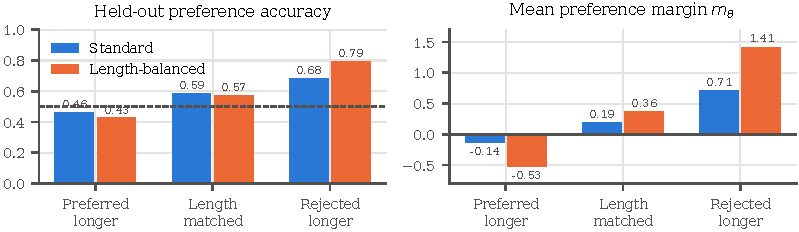
\includegraphics[width=\linewidth]{figures/t1_length_strata}
  \caption{\todo{caption}}
  \label{fig:t1-strata}
\end{figure}

% ~1.1 page
\section{Task 2: Proximal Policy Optimization}
\todo{standard continuation diagnostics, clipping study (define the stability statistic: Grad CV = std/mean of the
policy gradient norm across the 8 fork updates), KL-pressure study, qualitative examples}

\begin{figure}[t]
  \centering
  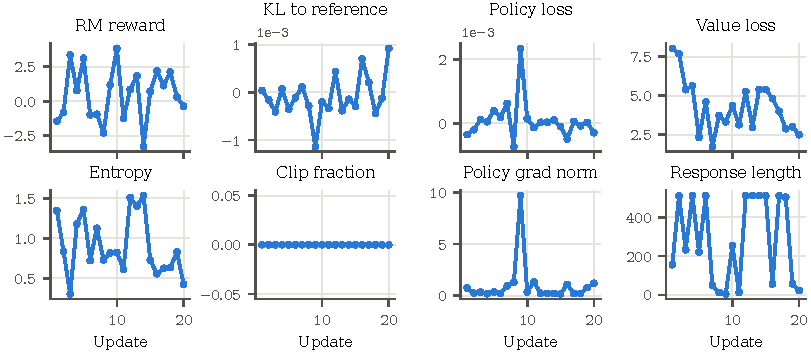
\includegraphics[width=\linewidth]{figures/t2_ppo_trajectories}
  \caption{\todo{caption}}
  \label{fig:t2-traj}
\end{figure}

\begin{table}[t]
  \centering
  \resizebox{\linewidth}{!}{\begin{tabular}{lrrrrrrrrr}
\toprule
Condition & $\epsilon$ & $\beta_\text{KL}$ & Cache aff. & RM score & KL$_\text{seq}$ & Entropy & Length & Grad CV & Clip frac. \\
\midrule
Midpoint (start) & 0.20 & 0.10 & -- & 1.656 & -0.0017 & 0.998 & 285 & -- & -- \\
Standard, 20 upd. & 0.20 & 0.10 & -- & 1.729 & 0.0124 & 1.000 & 284 & -- & -- \\
\midrule
$\epsilon{=}0.05$ & 0.05 & 0.10 & 0.168 & 1.766 & -0.0047 & 1.010 & 294 & 0.71 & 0.000 \\
$\epsilon{=}0.20$ & 0.20 & 0.10 & 0.056 & 1.766 & -0.0047 & 1.010 & 294 & 0.71 & 0.000 \\
$\epsilon{=}0.50$ & 0.50 & 0.10 & 0.030 & 1.766 & -0.0047 & 1.010 & 294 & 0.71 & 0.000 \\
\midrule
$\beta_\text{KL}{=}0$ & 0.20 & 0.00 & -- & 1.622 & -0.0094 & 1.002 & 285 & 0.69 & 0.000 \\
$\beta_\text{KL}{=}0.20$ & 0.20 & 0.20 & -- & 1.691 & 0.0014 & 1.007 & 295 & 0.72 & 0.000 \\
\bottomrule
\end{tabular}
}
  \caption{\todo{caption}}
  \label{tab:t2}
\end{table}

% ~1.1 page
\section{Task 3: Group Relative Policy Optimization}
\todo{standard continuation, group-size study (difficulty bins = tertiles of per-prompt mean cached reward),
canonical vs Dr.~GRPO, qualitative examples}

\begin{figure}[t]
  \centering
  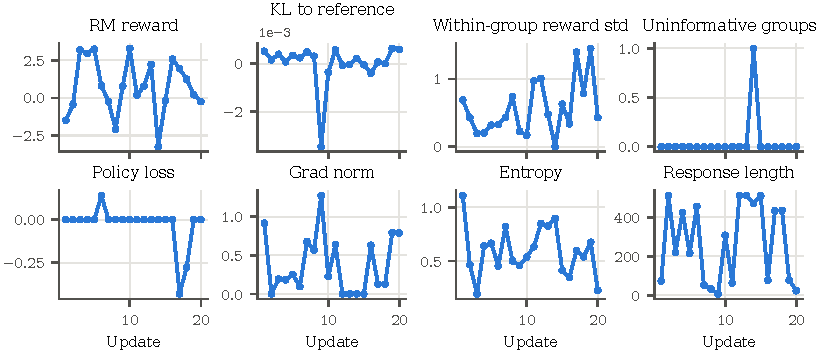
\includegraphics[width=\linewidth]{figures/t3_grpo_trajectories}
  \caption{\todo{caption}}
  \label{fig:t3-traj}
\end{figure}

\begin{table}[t]
  \centering
  \resizebox{\linewidth}{!}{\begin{tabular}{rr rrr rr rr rr}
\toprule
 & & \multicolumn{3}{c}{All prompts} & \multicolumn{2}{c}{Easy} & \multicolumn{2}{c}{Medium} & \multicolumn{2}{c}{Hard} \\
\cmidrule(lr){3-5}\cmidrule(lr){6-7}\cmidrule(lr){8-9}\cmidrule(lr){10-11}
$K$ & Groups & Inform. & Std & Var$(A)$ & Inform. & Std & Inform. & Std & Inform. & Std \\
\midrule
2 & 96 & 0.938 & 0.385 & 0.937 & 1.000 & 0.248 & 0.969 & 0.412 & 0.844 & 0.493 \\
4 & 48 & 0.958 & 0.541 & 0.958 & 1.000 & 0.410 & 1.000 & 0.552 & 0.875 & 0.661 \\
8 & 24 & 0.958 & 0.619 & 0.958 & 1.000 & 0.495 & 1.000 & 0.599 & 0.875 & 0.763 \\
\bottomrule
\end{tabular}
}
  \caption{\todo{caption}}
  \label{tab:t3-k}
\end{table}

\begin{table}[t]
  \centering
  \resizebox{\linewidth}{!}{\begin{tabular}{lrrrrrrr}
\toprule
 & \multicolumn{4}{c}{Held-out} & \multicolumn{3}{c}{Per-completion grad norm} \\
\cmidrule(lr){2-5}\cmidrule(lr){6-8}
Normalization & RM score & KL$_\text{seq}$ & Length & Trunc. & Short & Medium & Long \\
\midrule
Canonical ($1/T_k$) & 1.610 & 0.0172 & 282 & 0.095 & 0.270 & 0.193 & 0.112 \\
Dr.~GRPO & 1.721 & 0.0324 & 288 & 0.070 & 0.023 & 0.052 & 0.063 \\
\bottomrule
\end{tabular}
}
  \caption{\todo{caption}}
  \label{tab:t3-norm}
\end{table}

\begin{figure}[t]
  \centering
  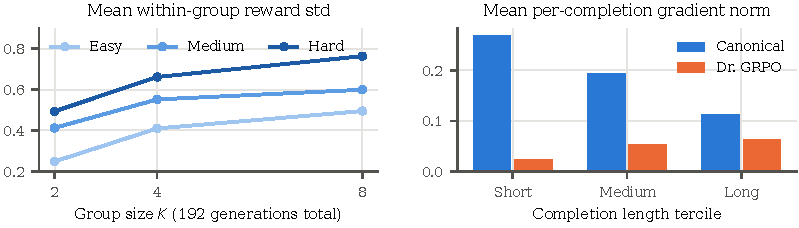
\includegraphics[width=\linewidth]{figures/t3_groupsize_normalization}
  \caption{\todo{caption}}
  \label{fig:t3-k-norm}
\end{figure}

% ~1.2 page
\section{Task 4: Safety calibration}
\todo{rates, category behaviour, manual audit agreement, disagreement examples (policy vs judge error)}

\begin{table}[t]
  \centering
  \resizebox{\linewidth}{!}{\begin{tabular}{lrrrrrrr}
\toprule
 & \multicolumn{3}{c}{Safe prompts ($n{=}250$)} & \multicolumn{2}{c}{Unsafe prompts ($n{=}200$)} & & \\
\cmidrule(lr){2-4}\cmidrule(lr){5-6}
Policy & Answer & Over-ref. & Any ref.$^\dagger$ & Unsafe comp. & Just. ref. & Ambig. & Length \\
\midrule
SFT & 0.572 & 0.000 & 0.416 & 0.000 & 0.885 & 0.000 & 108 \\
DPO & 0.572 & 0.000 & 0.420 & 0.000 & 0.865 & 0.000 & 109 \\
PPO & 0.576 & 0.000 & 0.412 & 0.000 & 0.880 & 0.000 & 108 \\
GRPO & 0.572 & 0.000 & 0.416 & 0.000 & 0.875 & 0.000 & 108 \\
\bottomrule
\end{tabular}
}
  \caption{\todo{caption; define the derived "Any ref." column marked with a dagger}}
  \label{tab:t4}
\end{table}

\begin{table}[t]
  \centering
  \resizebox{\linewidth}{!}{\begin{tabular}{l rrrrr r}
\toprule
Manual $\downarrow$ / AI judge $\rightarrow$ & Safe ans. & Just. ref. & Unsafe comp. & Over-ref. & Ambig. & Total \\
\midrule
Safe ans. & 43 & 7 & 0 & 0 & 0 & 50 \\
Just. ref. & 8 & 109 & 0 & 0 & 0 & 117 \\
Unsafe comp. & 0 & 0 & 0 & 0 & 0 & 0 \\
Over-ref. & 9 & 49 & 0 & 0 & 0 & 58 \\
Ambig. & 12 & 3 & 0 & 0 & 0 & 15 \\
\midrule
\multicolumn{7}{l}{Agreement 0.633, Cohen's $\kappa$ 0.385; safe 0.417, unsafe 0.850; $n{=}240$ pairs (116 distinct)} \\
\bottomrule
\end{tabular}
}
  \caption{\todo{caption}}
  \label{tab:t4-audit}
\end{table}

\begin{figure}[t]
  \centering
  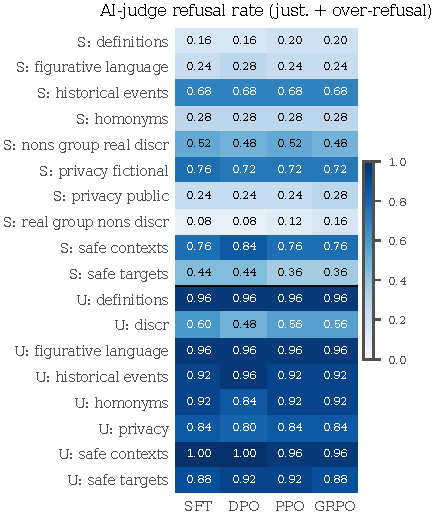
\includegraphics[width=0.55\linewidth]{figures/t4_category_refusal}
  \caption{\todo{caption}}
  \label{fig:t4-cat}
\end{figure}

% ~1.1 page
\section{Task 5: RLVR versus RLAIF}
\todo{in-domain, controlled diagnostics ($S_\text{reason}$, $S_\text{outcome}$), transfer, qualitative examples,
feedback-source discussion}

\begin{table}[t]
  \centering
  \resizebox{\linewidth}{!}{\begin{tabular}{l rrrr rrrr r}
\toprule
 & \multicolumn{4}{c}{GSM8K ($n{=}300$)} & \multicolumn{4}{c}{SVAMP transfer ($n{=}100$)} & \\
\cmidrule(lr){2-5}\cmidrule(lr){6-9}
Policy & Acc & Format & Length & Win vs SFT (ties) & Acc & Format & Length & Win vs SFT (ties) & $\Delta$Acc \\
\midrule
SFT & 0.273 & 0.353 & 275 & -- & 0.420 & 0.550 & 163 & -- & +0.147 \\
RLVR & 0.293 & 0.363 & 276 & 0.503 (290) & 0.460 & 0.580 & 164 & 0.530 (78) & +0.167 \\
RLAIF & 0.290 & 0.363 & 277 & 0.500 (292) & 0.480 & 0.620 & 164 & 0.535 (79) & +0.190 \\
\bottomrule
\end{tabular}
}
  \caption{\todo{caption}}
  \label{tab:t5}
\end{table}

\begin{table}[t]
  \centering
  \resizebox{\linewidth}{!}{\begin{tabular}{l rrr rrr}
\toprule
 & \multicolumn{3}{c}{Exact verifier} & \multicolumn{3}{c}{AI pairwise judge} \\
\cmidrule(lr){2-4}\cmidrule(lr){5-7}
Clean correct vs \ldots & Better & Tie & Wrong & Better & Tie & Wrong \\
\midrule
Reasoning corrupted & 0.00 & 1.00 & 0.00 & 0.00 & 1.00 & 0.00 \\
Wrong final answer & 1.00 & 0.00 & 0.00 & 0.00 & 1.00 & 0.00 \\
Persuasive filler & 0.00 & 1.00 & 0.00 & 0.00 & 0.75 & 0.25 \\
Gold-number distractor & 1.00 & 0.00 & 0.00 & 0.25 & 0.70 & 0.05 \\
\midrule
\multicolumn{7}{l}{$S_\text{reason}$: verifier 0.00, judge 0.00; $S_\text{outcome}$: verifier 1.00, judge 0.00; judge parse fallback 0.00 ($n{=}80$)} \\
\bottomrule
\end{tabular}
}
  \caption{\todo{caption}}
  \label{tab:t5-diag}
\end{table}

\begin{figure}[t]
  \centering
  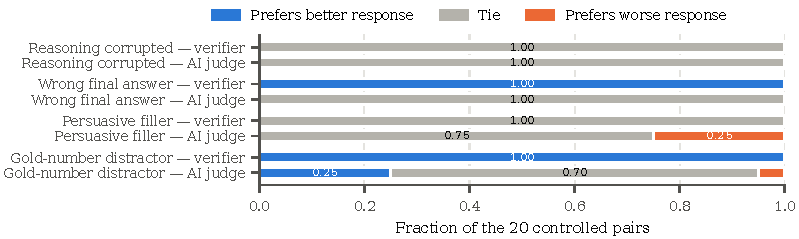
\includegraphics[width=\linewidth]{figures/t5_diagnostics}
  \caption{\todo{caption}}
  \label{fig:t5-diag}
\end{figure}

% ~0.8 page
\section{Cross-task discussion}
\todo{preference strength vs drift; offline vs online; optimization bias; safety calibration; reward-source design}

% ~0.3 page
\section{Conclusion}
\todo{conclusion}

% References do not count toward the 8 pages.
\begin{thebibliography}{9}
\bibitem{rafailov2023} \todo{Rafailov et al., 2023}
\bibitem{schulman2017} \todo{Schulman et al., 2017}
\bibitem{ouyang2022} \todo{Ouyang et al., 2022}
\bibitem{shao2024} \todo{Shao et al., 2024}
\bibitem{liu2025} \todo{Liu et al., 2025}
\bibitem{rottger2023} \todo{R\"ottger et al., 2023}
\bibitem{deepseek2025} \todo{DeepSeek-AI et al., 2025}
\bibitem{lee2024} \todo{Lee et al., 2024}
\end{thebibliography}

\end{document}
